\documentclass{llncs}
\usepackage{makeidx}  % allows for indexgeneration
\usepackage[utf8]{inputenc}

% color in codes
\usepackage{listings}
\usepackage{color}

\definecolor{mygreen}{rgb}{0,0.6,0}
\definecolor{mygray}{rgb}{0.5,0.5,0.5}
\definecolor{mymauve}{rgb}{0.58,0,0.82}

\lstset{ 
  backgroundcolor=\color{white},   % choose the background color; you must add \usepackage{color} or \usepackage{xcolor}; should come as last argument
  basicstyle=\footnotesize,        % the size of the fonts that are used for the code
  breakatwhitespace=false,         % sets if automatic breaks should only happen at whitespace
  breaklines=true,                 % sets automatic line breaking
  captionpos=b,                    % sets the caption-position to bottom
  commentstyle=\color{mygreen},    % comment style
  deletekeywords={...},            % if you want to delete keywords from the given language
  escapeinside={\%*}{*)},          % if you want to add LaTeX within your code
  extendedchars=true,              % lets you use non-ASCII characters; for 8-bits encodings only, does not work with UTF-8
%  firstnumber=1000,                % start line enumeration with line 1000
%  frame=single,	                   % adds a frame around the code
  keepspaces=true,                 % keeps spaces in text, useful for keeping indentation of code (possibly needs columns=flexible)
  keywordstyle=\color{blue},       % keyword style
  language=Octave,                 % the language of the code
  morekeywords={*,...},            % if you want to add more keywords to the set
%  numbers=left,                    % where to put the line-numbers; possible values are (none, left, right)
  numbersep=5pt,                   % how far the line-numbers are from the code
  numberstyle=\tiny\color{mygray}, % the style that is used for the line-numbers
  rulecolor=\color{black},         % if not set, the frame-color may be changed on line-breaks within not-black text (e.g. comments (green here))
  showspaces=false,                % show spaces everywhere adding particular underscores; it overrides 'showstringspaces'
  showstringspaces=false,          % underline spaces within strings only
  showtabs=false,                  % show tabs within strings adding particular underscores
%  stepnumber=2,                    % the step between two line-numbers. If it's 1, each line will be numbered
  stringstyle=\color{mymauve},     % string literal style
  tabsize=2,	                   % sets default tabsize to 2 spaces
  title=\lstname                   % show the filename of files included with \lstinputlisting; also try caption instead of title
}
%
\usepackage{graphicx}
\usepackage{hyperref} % use \href{}{}

\begin{document}

\pagestyle{headings}  % switches on printing of running heads
% \addtocmark{} % additional mark in the TOC

%\tableofcontents

\title{Proyecto Final de Sistemas de Recuperación de Información}

\titlerunning{Sistema de Recuperación de Información}  % abbreviated title (for running head)
%                                     also used for the TOC unless
%                                     \toctitle is used
%
\author{Karel Díaz Vergara, Alben Luis Urquiza Rojas}
%
\authorrunning{Karel Díaz y Alben Urquiza} % abbreviated author list (for running head)

%%%% list of authors for the TOC (use if author list has to be modified)
%\tocauthor{Karel Díaz Vergara, Alben Luis Urquiza Rojas}

\institute{Universidad de La Habana, Cuba}

\maketitle              % typeset the title of the contribution

\begin{abstract}
The world is becoming more and more computerized. Over time, more people and more services will be found on the internet. Ways are needed to make interaction and communication between people and these services easy. And what better way to do this than Information Search and Retrieval (IRS). When a user needs something, he makes a query in an IRS, and it will be answered with a page or web resource where the solution to that query can be found. To develop our IRS, we use the vector model, supporting on user feedback and using word embedding technic to represent words through numbers. This field will continue to be an important part of Computer Science and to which many studies and efforts will be devoted in future.
\keywords{sistema recuperación de la información, SRI, modelo vectorial, word embedding}
\end{abstract}
%
\section{Introducción}

La Búsqueda y Recuperación de Información, llamada en inglés \textbf{Information Search and Retrieval (ISR)}, es la ciencia de la búsqueda de información en documentos electrónicos y cualquier tipo de colección documental digital, encargada de la búsqueda dentro de estos mismos, búsqueda de metadatos que describan documentos, o también la búsqueda en bases de datos relacionales, ya sea a través de internet, una intranet, y como objetivo realiza la recuperación en textos, imágenes, sonido o datos de otras características, de manera pertinente y relevante.

La recuperación de información es un estudio interdisciplinario. Cubre tantas disciplinas que eso genera normalmente un conocimiento parcial desde tan solo una u otra perspectiva. Algunas de las disciplinas que se ocupan de estos estudios son la psicología cognitiva, la arquitectura de la información, diseño de la información, inteligencia artificial, lingüística, semiótica, informática, biblioteconomía, archivística y documentación.

Un proceso de recuperación de información comienza cuando un usuario hace una consulta al sistema. Una consulta a su vez es una afirmación formal de la necesidad de una información. En la recuperación de información una consulta no identifica únicamente a un objeto dentro de la colección. De hecho varios objetos pueden ser respuesta a una consulta con diferentes grados de relevancia.

Un objeto es una identidad que está representada por información en una base de datos. En dependencia de la aplicación estos objetos pueden ser archivos de texto, imágenes, audio, mapas, videos, etc. Muy a menudo los documentos no están almacenados en el sistema de recuperación de información, sino que están representados lógicamente.

La mayoría de los sistemas de recuperación de información computan un ranking para saber cuán bien cada objeto responde a la consulta, ordenando los objetos de acuerdo a su valor de ranking. Los objetos con mayor ranking son mostrados a los usuarios y el proceso puede tener otras iteraciones si el usuario desea refinar su consulta.

\subsection{Motor de Búsqueda}

El proyecto está dividido en dos aplicaciones, la interfaz gráfica (\textit{search\_engine\_interface}) desarrollada en VueJs, por la cual se realizan las consultas que se hacen a la segunda aplicación(\textit{info\_retrieval\_model}) desarrollada con el framework fast api.

\textbf{Repositorio en github: \url{https://github.com/Karelito00/search_engine/tree/develop}}

\subsubsection{Frontend / Interfaz Gráfica} \hfill

\textbf{Requerimientos:} \\
- vue \\
- vue-router \\
- yarn/npm \\

\textbf{Instalación}
\begin{lstlisting}[language=bash]
$ cd search_engine_interface/
$ yarn install
\end{lstlisting}

\textbf{Run:}
\begin{lstlisting}[language=bash]
$ cd search_engine_interface/
$ yarn serve
\end{lstlisting}

\subsubsection{Backend / Modelo de recuperación de la información} \hfill

\textbf{Requerimientos:} \\
- python3 \\
- fastapi \\
- hypercorn \\
- sklearn \\
- numpy \\
- scipy \\
- nltk \\

\textbf{Run:}
\begin{lstlisting}[language=bash]
$ cd info_retrieval_model/
$ hypercorn main.py --reload
\end{lstlisting}

\subsection{Esquema del flujo del motor de búsqueda:}

\begin{center}
	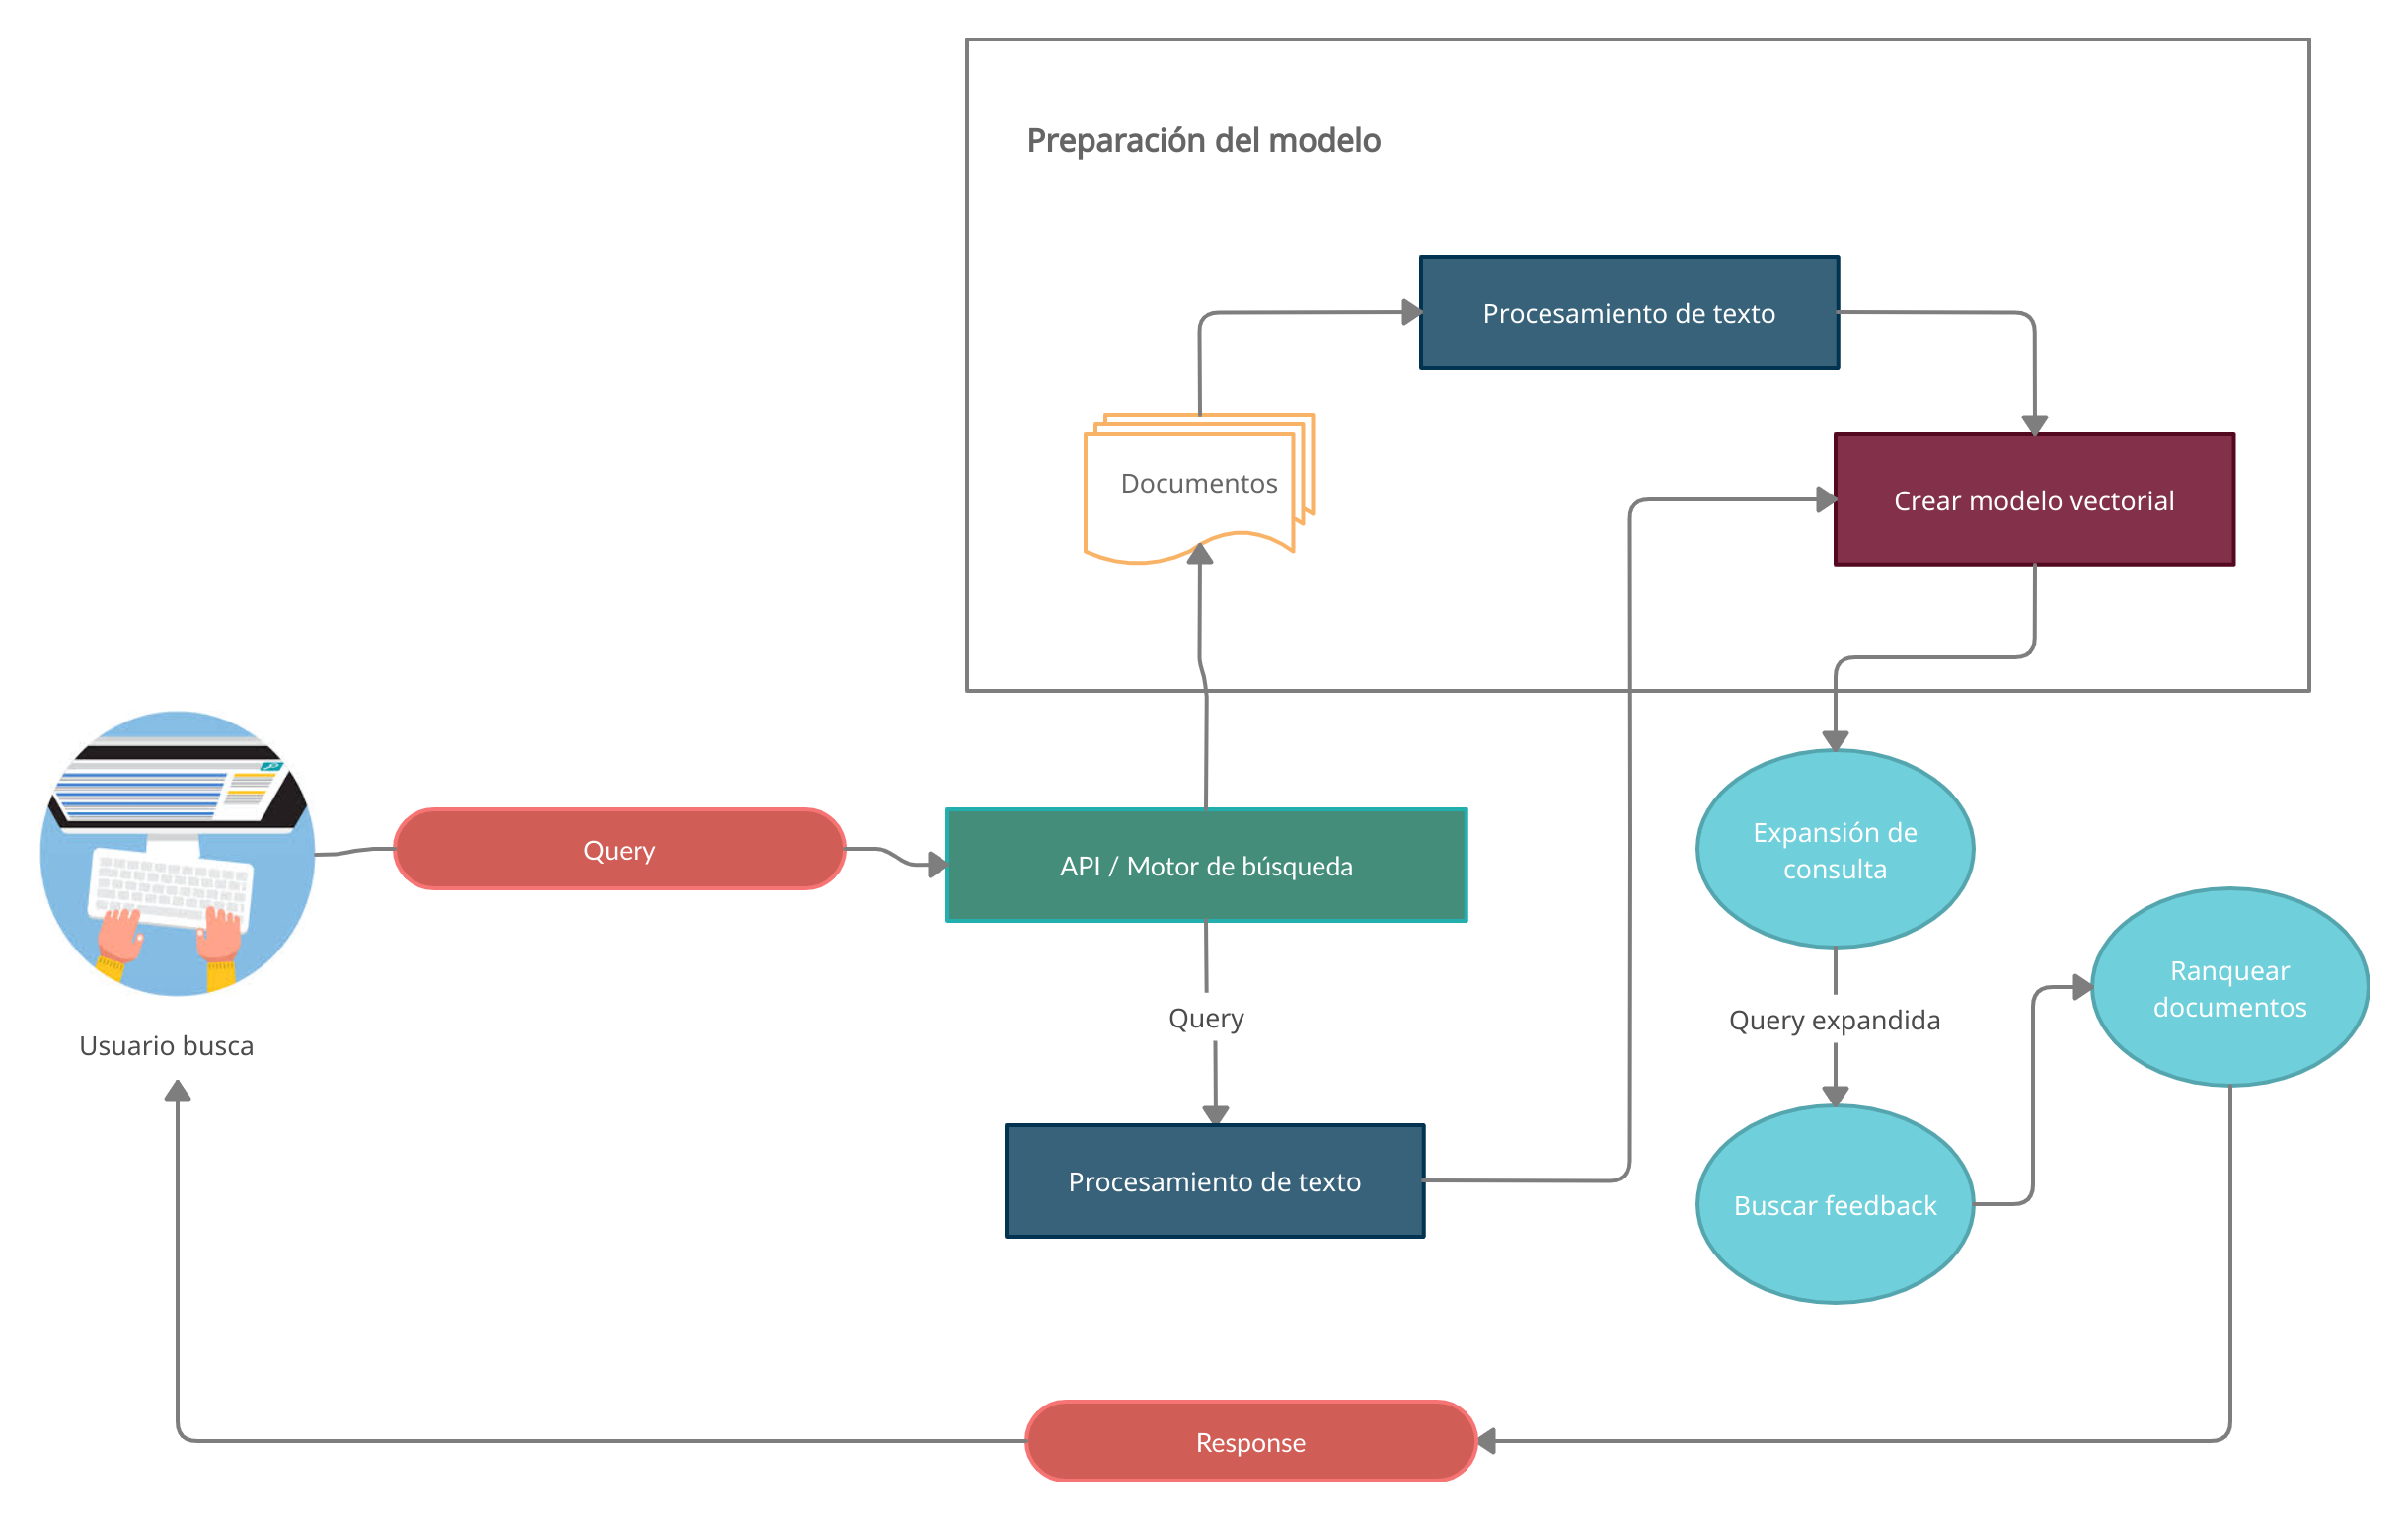
\includegraphics[scale=0.15]{../application-flow.jpg}\\
\end{center}

\subsection{Preparación del modelo}

Se utilizaron dos colecciones de datos \href{http://ir.dcs.gla.ac.uk/resources/test_collections/npl/}{npl} y \href{http://ir.dcs.gla.ac.uk/resources/test_collections/lisa/}{LISA-collection}, para cada una de estas se creó una carpeta que contiene todos los documentos en archivos diferentes, para poder ser importados en la aplicación de forma fácil, con la clase \textbf{FileTools} tenemos un método para obtener el path de todos los documentos en un directorio, y un método para obtener el contenido de un archivo, de esta forma podemos cargar cada test-collection.

\begin{lstlisting}[language=Python]
def initialize(root_path = "."):
    # Provide the collection path
    # news-group collection
    ft = FileTools(f"{root_path}/collections/news-group")

    # docs-lisa collection
    # ft = FileTools(f"{root_path}/collections/docs-lisa")

    docs = ft.get_documents()
    return VectorialModel(map(lambda doc: ft.read_document(doc), docs))
\end{lstlisting}

\subsection{Preprocesamiento de texto}

Luego vamos a crear nuestro modelo vectorial, cada documento pasa primero por un filtro de preprocesamiento de texto, de manera tal que le aplicamos las siguientes operaciones:

\begin{itemize}
	\item Expandimos contracciones
	\item Convertimos las palabras a minúscula
	\item Removemos los signos de puntuación
	\item Removemos las palabras que contengan dígitos
	\item Removemos las stopwords(aquellas palabras que no proveen ninguna información útil para decidir en que categoría se debe clasificar el texto. Dígase: preposiciones, conjunciones, etc.)
	\item Aplicamos lematización. Lematización es un proceso lingüístico que consiste en, dada una forma flexionada (es decir, en plural, en femenino, conjugada, etc.), hallar el lema correspondiente. El lema es la forma que por convenio se acepta como representante de todas las formas flexionadas de una misma palabra. Es decir, el lema de una palabra es la palabra que nos encontraríamos como entrada en un diccionario tradicional: singular para sustantivos, masculino singular para adjetivos, infinitivo para verbos.
\end{itemize}


Luego de esto digamos que tenemos un arreglo de cadenas, donde a cada cadena le llamaremos término.


\subsection{Build del modelo vectorial}


Guardamos para cada término la cantidad de documentos diferentes en los que aparece y además calculamos por cada documento la frecuencia normalizada de cada término($tf_i$).

$$ tf_i = \frac{f_i} {maxfrec} $$

\begin{lstlisting}[language=Python]
def build_freq(self):
    freq = {}
    for term in self.terms:
        if(freq.__contains__(term) == False):
            freq[term] = 1
        else:
            freq[term] += 1
    self.freq = Vector(freq)

def calculate_tfi(self):
    tfi = {}
    max_freq = max(self.freq.values())

    for term in self.freq:
        tfi[term] = self.freq.vector[term] / max_freq
    self.tfi = Vector(tfi)
\end{lstlisting}

La variable $maxfrec$ corresponde a la frecuencia del término que más se repite en el documento. Esta frecuencia normalizada se realiza con el objetivo de que si un documento es igual que otro, pero con los mismos términos repetidos $x$ veces no se le reste importancia al que menos frecuencia tiene, ya que los dos tendrían la misma importancia.

\begin{lstlisting}[language=Python]
def __init__(self, docs):
    self.term_universe = {}
    self.docs = []
    self.feedback = Feedback()
    self.word_embedding = WordEmbedding("./core/word_embedding")
    for doc in docs:
        doc = Doc(doc)
        for term in doc.freq:
            if(self.term_universe.__contains__(term) == False):
                self.term_universe[term] = 1
            else:
                self.term_universe[term] += 1
        self.docs.append(doc)

    self.calculate_idf()
    self.calculate_weight_of_docs()
\end{lstlisting}

Ya luego pasamos a calcular la frecuencia inversa de cada término del vocabulario y con ello podemos obtener los pesos de cada término por documento.

$$idf_i = log(\frac{N}{n_i})$$
$$ w_i = tf_i * idf_i$$

Donde $N$ es la cantidad de documentos que tiene nuestro test collection y $n_i$ corresponde a la cantidad de documentos en los que aparece el $i$-ésimo término de nuestro vocabulario.

Ya tenemos nuestro modelo construido, podemos proceder a realizarle consultas

\subsection{Realizar una query:}

Mediante fastapi recibimos los requests que hace nuestra interfaz de usuario:

\begin{lstlisting}[language=Python]
@app.get("/query")
def query_docs(value: str = ""):
    documents = vm.query(value)
    return prepare_output(documents)
\end{lstlisting}

Donde value sería el texto de nuestra query, entonces las queries las trataremos como si fueran documentos, que quiere decir esto, todas pasarán primero por un preprocesamiento de texto donde obtenemos un arreglo con sus términos y entonces calculamos la frecuencia normalizada para cada término, así como sus pesos($w_i$)


Como podemos ver en la clase \textbf{Doc} a la hora de calcular el peso de cada término($w_i$) hacemos una pequeña modificación a la fórmula, añadiendo un valor $A$ que permite amortiguar la contribución de la frecuencia de cada término, los valores más comunes son 0.4 y 0.5, nosotros utilizamos $A = 0.4$


$$ w_i = (A + (1 - A) * tf_i) * idf_i $$


Entonces ya que tenemos los pesos de la consulta, bastaría entonces con ranquear los documentos utilizando la fórmula de similitud del coseno:


$$ sim(d_j, q) = \frac{\sum^n w_{i,j} * w_{i,q}}{\sqrt{\sum^n w^2_{i,j}} * \sqrt{\sum^n w^2_{i,q}}} $$


Es decir para cada término del vocabulario multiplicamos los pesos en el documento $j$ y en la query.

\begin{lstlisting}[language=Python]
def correlation(self, vector_a, vector_b):
    sum_t = 0
    max_vector = vector_a if len(vector_a) >= len(vector_b) else vector_b
    min_vector = vector_a if len(vector_a) < len(vector_b) else vector_b
    for term in min_vector:
        if(max_vector.__contains__(term)):
            sum_t += min_vector[term] * max_vector[term]

    if(sum_t < EPS):
        return 0
    if(vector_a.norm * vector_b.norm < EPS):
        return 100000
    return sum_t / (vector_a.norm * vector_b.norm)
\end{lstlisting}

Lo que hacemos en ese código es escoger el documento que tiene menor cantidad de términos(entre el documento $j$ y la query) así nos ahorramos costo operacional, ya que si un término no aparece en uno de los documentos la multiplicación es cero.


Al final verificamos que la multiplicación de las normas sea mayor que cero para que no se nos indefina nuestra correlación


¿Cuándo la norma de un documento puede ser cero?  
Esto solo ocurre si cada término del documento aparece en todos los demás documentos de nuestro test collection, ya que $N$ sería igual a $n_i$


Ahora que ya tenemos rankeados los documentos podemos devolverlos al frontend(para que sean mostrados al usuario), pero antes vamos a ver que mejoras implementamos.


\subsection{Añadiendo feedback/retroalimentación:}


En el frontend de nuestro proyecto añadimos la posibilidad de abrir cada documento, de forma tal que pueda revisarse el contenido de los documentos retornados y además la posibilidad de decir si es relevante o no. Por lo que tenemos la clase \textbf{Feedback}


La cual contiene dos métodos: \textbf{get\_feedback} y \textbf{set\_feedback}, entonces por cada documento que nos den feedback haciendo uso de un trie(trie es una estructura de datos para guardar cadenas, con costo lineal en tiempo con respecto al tamaño de la cadena) podemos insertar una query y en el nodo final tendremos un set con los índices de los documentos relevantes y otro set con los índices de los no relevantes, si en algún momento decimos que el documento \textit{d} era no relevante y ahora el usuario lo clasificó como relevante en esa query entonces lo eliminamos del set de no relevantes y lo añadimos en el de relevantes, y viceversa. El uso del trie es con el objetivo de evitar hacer hash a las query, hashes que luego puedan traer colisiones, ya que podemos tener muchísimas queries en feedback, este caso es posible.

\begin{lstlisting}[language=Python]
def set_feedback(self, query, feedback_type, doc_index):
    node = self.first_node
    for term in query.terms:
        if(node.mapp.__contains__(term) == False):
            node.mapp[term] = Node()
        node = node.mapp[term]

    if(feedback_type == 1):
        if(node.no_relevants.__contains__(doc_index)):
            node.no_relevants.remove(doc_index)
        node.relevants.add(doc_index)
    else:
        if(node.relevants.__contains__(doc_index)):
            node.relevants.remove(doc_index)
        node.no_relevants.add(doc_index)
\end{lstlisting}

Y ya luego para obtener el feedback es caminar por el trie, hasta llegar al final de la query en el caso de que exista y obtener los índices de los documentos no relevantes y relevantes.

\begin{lstlisting}[language=Python]
def get_feedback(self, query):
    node = self.first_node
    for term in query.terms:
        if(node.mapp.__contains__(term) == False):
            return None
        node = node.mapp[term]

    return [node.relevants, node.no_relevants]
\end{lstlisting}

¿Qué podemos hacer con esto?

\begin{lstlisting}[language=Python]
def get_feedback(self, query_doc):
    query_feedback = self.feedback.get_feedback(query_doc)
    if(query_feedback is None):
        return None
    relevants, no_relevants = query_feedback[0], query_feedback[1]
    qm = query_doc.wi

    sum_relev = functools.reduce(lambda a, b: a + self.docs[b].wi, relevants, Vector())
    sum_no_relev = functools.reduce(lambda a, b: a + self.docs[b].wi, no_relevants, Vector())

    b = 0 if len(relevants) == 0 else 0.75 / len(relevants)
    y = 0 if len(no_relevants) == 0 else 0.15 / len(no_relevants)
    qm = qm + (sum_relev * b) - (sum_no_relev * y)
    qm.calculate_norm()
        return qm
\end{lstlisting}

Pues creamos una nueva query, llamémosle $q_m$ y quedaría de la siguiente forma:


$$ q_m = q + \beta * d_r - \gamma * d_{nr} $$


Es decir tendremos nuevos pesos en los términos, sumamos los pesos de nuestra query base($q$) y luego por cada documento relevante sumamos el peso de cada término multiplicado por $\beta$, y por cada documento no relevante restamos el peso de cada término multiplicado por $\gamma$, los valores de $\beta$ y $\gamma$ que se utilizaron fueron $0.75$ y $0.15$ respectivamente.


El algoritmo en resumen lo que hace es darle mayor importancia a los términos más usados en los documentos considerados relevantes para los usuarios, y, por el contrario, los términos más usados en los documentos no relevantes se les da menor importancia.


Con este nuevo vector de pesos en nuestra query podemos ranquear los documentos y retornarlos, pero antes veamos como añadimos expansión de consultas.


\subsection{Expansión de consulta:}


Hasta ahora solo trabajamos con los términos de nuestro vocabulario, pero que pasa cuando el documento que buscamos no contiene los términos de nuestra query, porque resulta que son similares, ya sea porque son sinónimos o familias de palabras.


Aquí es donde las word embeddings juegan un papel importante.
¿Qué es word embeddings?
No es más que un conjunto de modelos de lenguaje y técnicas de aprendizaje en procesamiento del lenguaje natural en dónde las palabras o frases del lenguaje natural son representadas como vectores de números reales.


Al tener representada las palabras como vectores podemos saber que tan similares son dos palabras.


Entonces en nuestro proyecto, utilizamos un modelo pre-entrenado de \href{https://nlp.stanford.edu/projects/glove/}{glove}\cite{pennington2014glove}, específicamente el \textit{glove.6B} el cual contiene 400 mil términos, representados en vectores de 50, 100, 200 y 300 dimensiones.


Al momento de obtener una query, por cada término de \textit{q} que aparezca en las word embeddings de glove buscamos el término más similar, como hacemos esto, para cada término de glove, hallamos la distancia euclidiana entre este y el word embedding de \textit{q}, y nos quedamos con el de menor distancia.


Esto tiene una complejidad temporal de $O(N)$ (esto obviando el costo de hallar la distancia euclidiana entre dos puntos), cosa que estaríamos haciendo por cada término, algo lento si nuestra query tiene muchos términos diferentes.


Pero aquí entra \href{https://es.wikipedia.org/wiki/\%C3\%81rbol_kd}{KDTree}, es una estructura de datos de particionado del espacio que organiza los puntos en un Espacio euclídeo de K dimensiones. Entonces al cargar las word embeddings de glove creamos nuestro kdtree, y ya luego solo sería realizar las consultas.

\begin{lstlisting}[language=Python]
def find_similar_word_kdtree(self, embedes, count = 2):
    _, nearests = self.kd_tree.query([embedes], k = count)
    return [self.keys[nearests[0][1]]]
\end{lstlisting}

Utilizamos el KDTree ya implementado en \textit{sklearn}. Citando la documentación:  
\textit{"KD tree query time changes with D in a way that is difficult to precisely characterise. For small D (less than 20 or so) the cost is approximately O(D log N), and the KD tree query can be very efficient. For larger D, the cost increases to nearly O(D * N), and the overhead due to the tree structure can lead to queries which are slower than brute force."}

Traducción:
El tiempo de consulta del KD-tree cambia con respecto a \textbf{D} de una manera que es difícil de caracterizar con precisión. Para \textbf{D} pequeños (menos de 20 aproximadamente) el costo es de aproximadamente \textbf{O(D log N)}, y la consulta del KD-tree puede ser muy eficiente. Para \textbf{D} más grande, el costo aumenta a casi \textbf{O(D * N)}, y la sobrecarga debido a la estructura de árbol puede generar consultas que son más lentas que la fuerza bruta.


Sin embargo, en todos los casos que se probaron funcionó mucho más rápido que la fuerza bruta, en este proyecto utilizamos vectores de 300 dimensiones.


Ya tenemos para cada término de nuestra query la word embedding más similar, para identificar los términos de la expansión creamos un vector basado en estos word embeddings, un enfoque llamado average word embeddings (AWE), el cual le da el mismo peso a cada término de la query:


$$AWE(q) = \frac{1}{n} \sum_{w_i \in q} \vec{w_i}$$


Donde $\vec{w_i}$ corresponde al word embedding del término $wi$ que pertenece a la query, y $n$ es el número de términos diferentes que tiene la query $q$.


Kuzi et al(Saar Kuzi, "et al" es una expresión en latín que significa: y otros), propone el uso de closest term, el cual se mide por similitud del coseno entre nuestro vector AWE y el word embedding candidato a término de expansión. Los autores definen la función de puntación de esta forma:


$$ S(w, q) = exp^{\displaystyle{cos(\vec{w}, AWE(q))}} $$


Donde $\vec{w}$ sería el word embedding correspondiente al término $w$


Vamos a extender la fórmula AWE usando una estrategia basada en datos para combinar las word embeddings. La representación de nuestro vector IDF-AWE, es una representación de nuestra query generada por la combinación lineal de nuestros términos correspondientes a las word embeddings con sus IDF:


$$ IDF-AWE(q) = \frac{1}{\sum_{w_i \in q} IDF(w_i)} * \sum_{w_i \in q} IDF(w_i) * \vec{w_i}$$


Donde el IDF está calculado con respecto al vocabulario, IDF-AWE dará más importancia a términos de \textit{q} que son más específicos en el vocabulario. Para mantener la magnitud de los word embeddings, la suma de los vectores es multiplicada por la suma de los IDF de los términos que pertenecen a la query, de esta forma el vector IDF-AWE toma la misma magnitud que los words embeddings.

\begin{lstlisting}[language=Python]
# IDF-AWE(q) = ( 1 / sum (IDF(wordi) ) ) * sum( IDF(wordi) * wordi_vector )
# wordi is the word embedding of qi term of the query
def get_idf_awe(self, wordi_array):
    AWE_vector = np.zeros(self.word_embedding.vector_dimension, dtype=float)
    sum_IDF = 0
    embed_dict = self.word_embedding.embed_dict
    for val in wordi_array:
        sum_IDF +=  self.get_word_idf(val[1])
        AWE_vector += embed_dict[val[0]] * self.get_word_idf(val[1])

    return AWE_vector * ( 1 / sum_IDF )

def get_query_expansion(self, query_doc):
    wordi_array = []
    embed_dict = self.word_embedding.embed_dict
    for term in query_doc.terms:
        # word embeddings related with qi term
        if(embed_dict.__contains__(term)):
            wordi_array = wordi_array + [[self.word_embedding.find_similar_word_kdtree(embed_dict[term])[0], term]]
    idf_awe_vector = self.get_idf_awe(wordi_array)
    wordi_ranking = list(map(lambda val: [np.exp(spatial.distance.cosine(embed_dict[val[0]], idf_awe_vector)), val[0]], wordi_array))
    return list(map(lambda x: x[0], sorted(wordi_ranking, reverse=True)))
\end{lstlisting}

Entonces ya teniendo nuestro vector IDF-AWE y apoyándonos en la fórmula de similitud de arriba, nos quedamos con los 10 primeros word embeddings. Y los añadimos a nuestra query como términos de expansión y ahora si obtenemos feedback, calculamos los pesos nuevamente, y ranqueamos los documentos.

\section{Pruebas}
Para probar el algoritmo de recuperación de la información implementado se usaron algunas colecciones de pruebas predefinidas(a las cuales se hace referencia al principio del documento). A continuación se muestra una comparación entre el resultado obtenido por el algoritmo implementado y los documentos que según la colección de prueba utilizada son los más relevantes.

Para la colección de Lisa

\begin{tabular}{|p{2.5cm}|p{4.5cm}|p{4cm}|} \hline
Query number & Lisa response & Our information retrieval response \\ \hline
\#6 & 111 112 \textbf{113} 1100 1581 1582 \textbf{2090 2616} 2620 3647 \textbf{4155} 5066 5068 \textbf{5626 5627 5628} 5629 5631 & \textbf{5627 2090} 2886 5830 2593 \textbf{5626} 3103 \textbf{4155} 2722 3185 566 987 \textbf{113 5628} 988 5038 10 5343 \textbf{2616} 2618 \\ \hline
\#7 & 277 278 279 1277 1278 1769 2279 3265 3267 3450 3789 5220 5748 5778 & 2279 345 1278 1359 1277 3343 2351 5189 5778 1931 5748 704 5779 1924 2753 5931 4813 4731 359 215 \\ \hline
\#8 & 40 49 199 524 697 701 1043 1044 1190 1191 1534 1677 2039 2545 3045 3716 4485 4486 4499 4717 5011 5170 5533 5534 5723 5816 & 4469 39 2806 40 5506 3045 4478 5722 1044 4479 1191 3716 5530 4497 49 3942 1038 3744 78 1522 \\ \hline
\end{tabular} \\\\

Pruebas para la colección de npl

\begin{tabular}{|p{2.5cm}|p{4.5cm}|p{4cm}|} \hline
Query number & npl response & Our information retrieval response \\ \hline
\#1 & 1239  1502  4462  4569  5472  5502  6471  6480  6664  6824 7923  8150  8172  8277  9219  9859  9988 10081 10588 & 5502 7230 9859 8276 3885 6276 2236 8298 4861 4463 4533 10394 1828 10652 1756 720 7831 58 6635 1502 \\ \hline
\#4 & 402  2546  4180  4419  5435  5437  5440  8099 10162 11178 & 5440 8534 10051 8643 4830 10162 7267 3035 5015 1835 4256 4306 4316 4594 4807 3956 2673 5263 5437 2936 \\ \hline
\#13 & 281  1337  1732  2085  2209  2458  2459  2463  3297  3398 3522  3641  3852  3984  4080  4454  4627  5045  5276  5368 5477  5743  5873  5980  6088  6273  6530  6534  6548  6549 6622  6909  6974  7073  7111  7176  7262  7374  7702  7709 7823  7908  8024  8136  8448  8563  8567  8960  9183  9423 9433  9434  9698 10192 10363 10487 10634 11037 11053 & 8346 5873 3631 10039 5250 8464 2312 4454 11053 2458 11312 3398 1167 9183 3401 1852 10755 1612 4079 \\ \hline
\end{tabular}

\section{Análisis crítico}


Entre las ventajas del modelo que implementamos, podemos decir que es bastante rápido a la hora de procesar un gran volumen de documentos, además de que se basa en las métricas TF-IDF para darle peso a los términos de los documentos.  
Pero no todo es bueno, algo que tiene el modelo vectorial es que cuando haces una query para recuperar un documento tiene que tener al menos un término en común con el documento, de lo contrario la similitud por coseno será igual a cero, este problema le dimos solución usando las word embeddings, las cuales nos permiten encontrar términos similares que quizás no estaban en la query.  
Otra desventaja es que si queremos añadir documentos en tiempo de ejecución, tendremos que recalcular el modelo completamente, algo que nos costaría un poco de tiempo.  
Es decir, este modelo está hecho para motores de búsquedas estáticos, o poco mutantes.

\subsection{Posibles mejoras}

Entre las posibles mejoras para trabajos futuros está utilizar el modelo pre-entrenado de tensorflow ELMO(Embeddings from Language Model), el cual es un modelo para representar una secuencia de palabras como una secuencia de vectores y lo podemos utilizar para dado un texto obtener una palabra que se relacione con el contexto, algo así como sacar la idea central, lo que se conoce como CBOW(Continuos Bag of Words).

Quizás implementar el modelo probabilístico :)

\section{Galería}

\begin{center}
	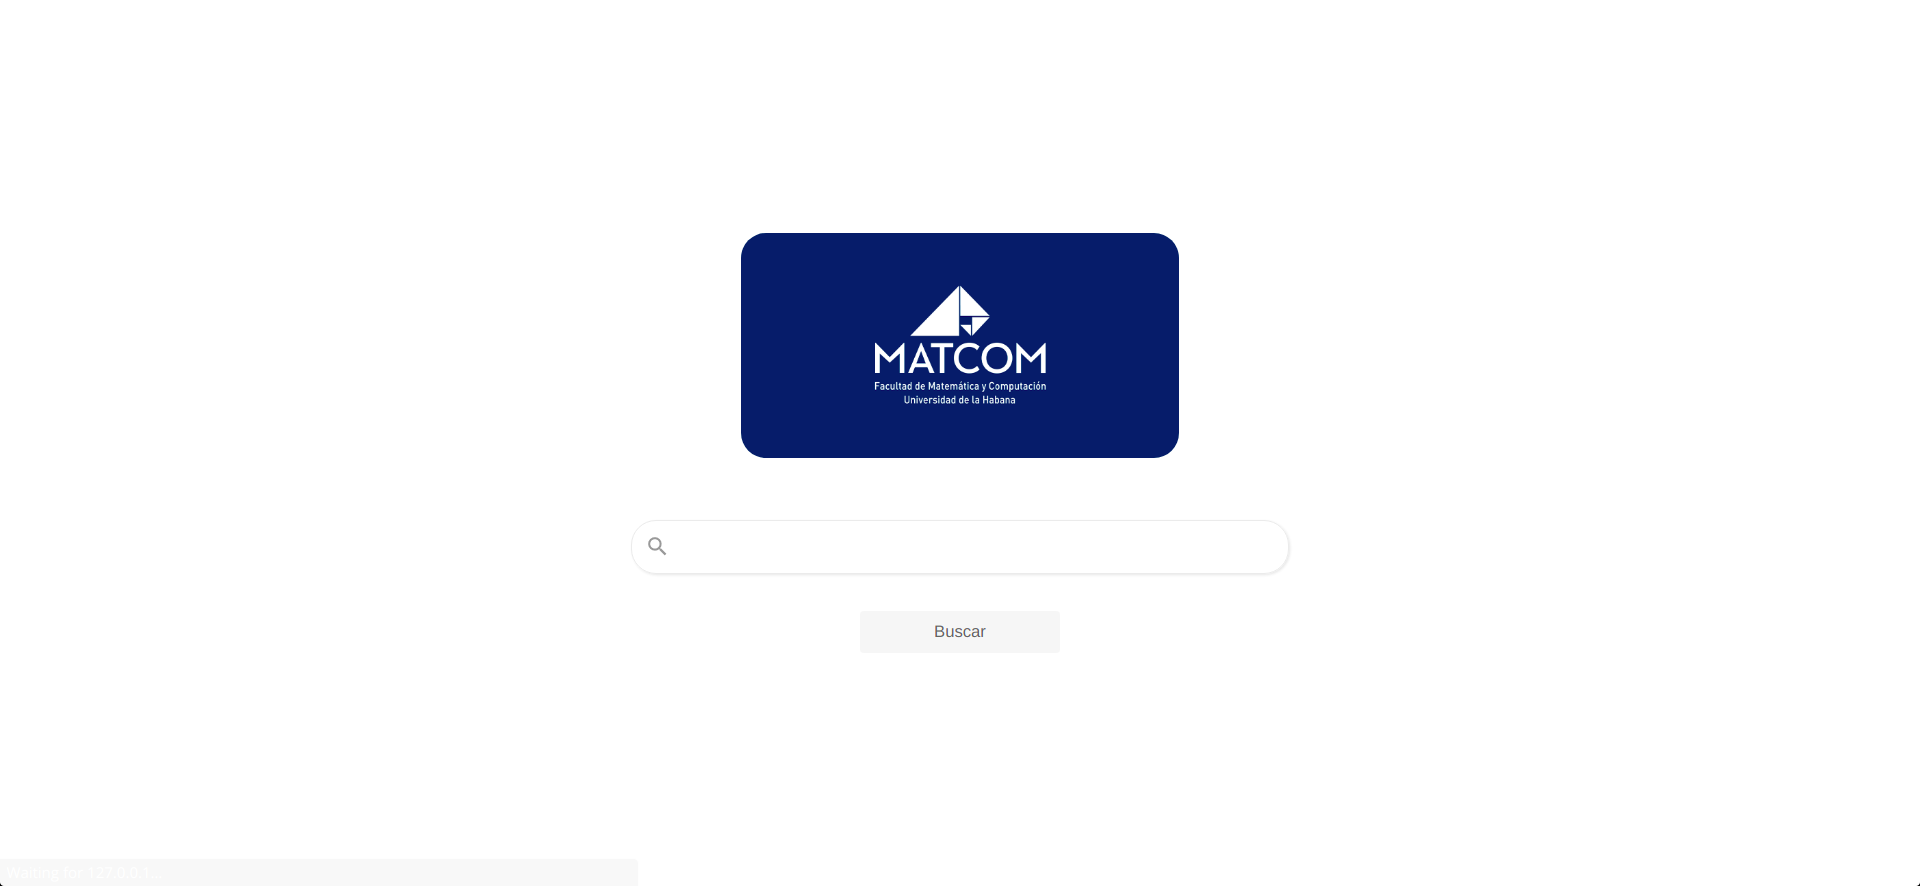
\includegraphics[scale=0.18]{../image-2.png}\\
	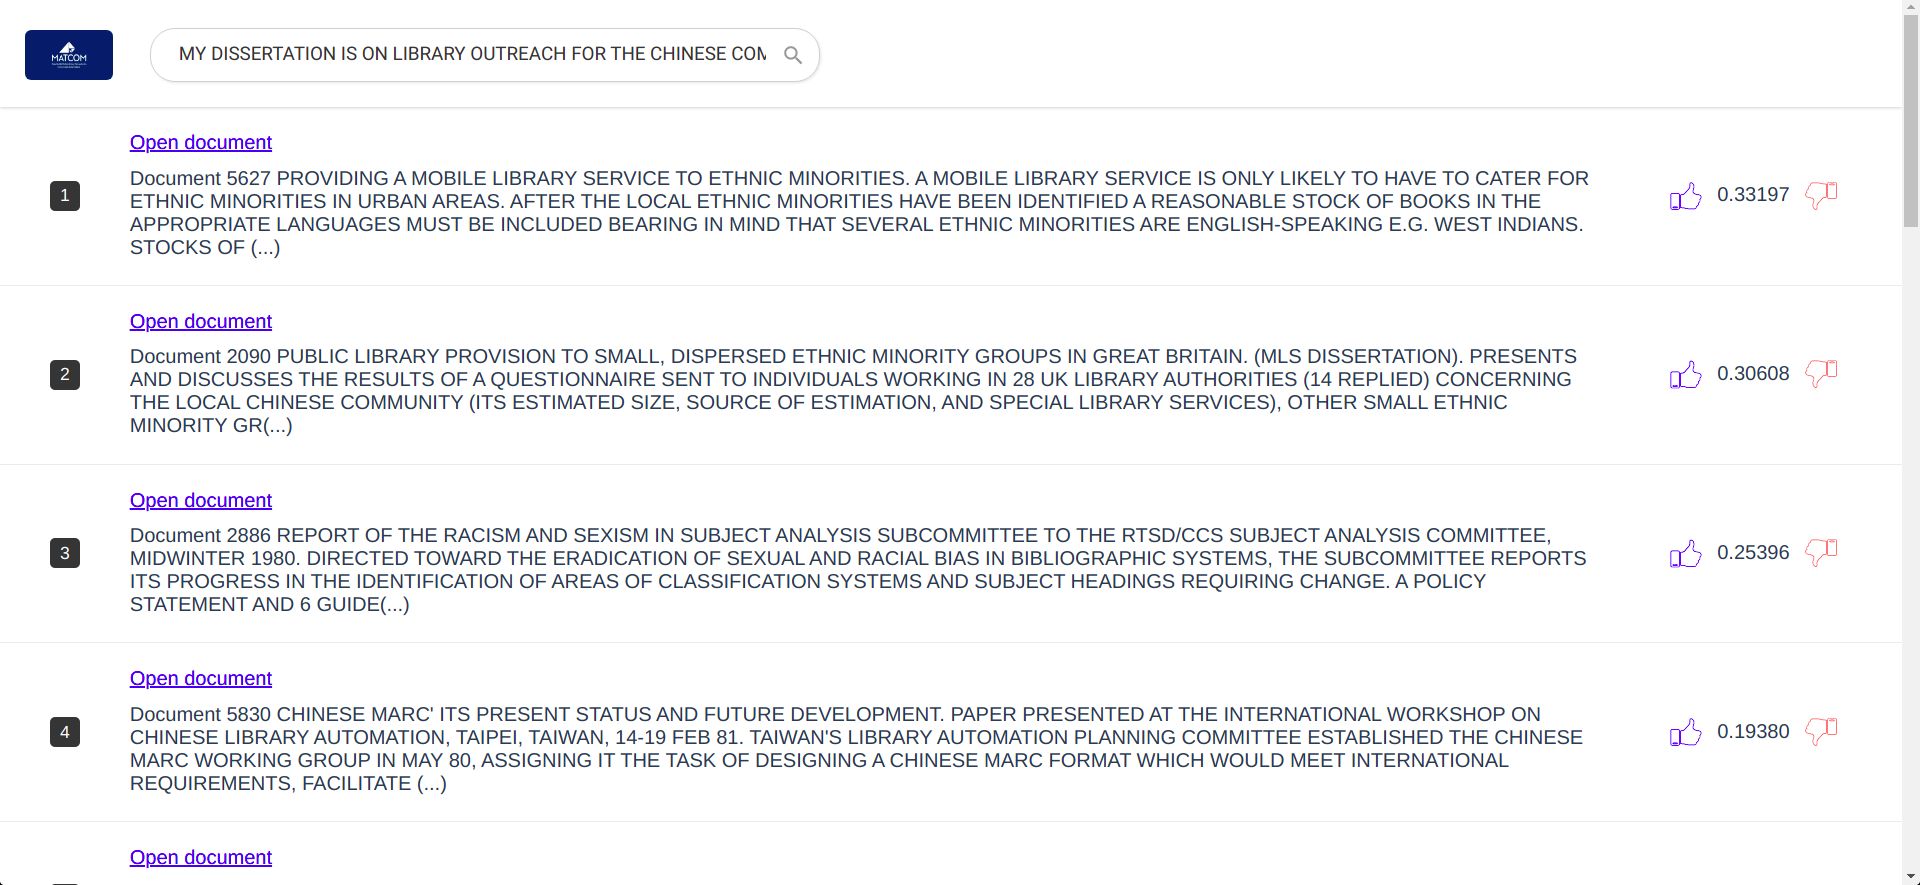
\includegraphics[scale=0.2]{../image-1.png}\\
	
	\href{https://www.loom.com/share/6d941e0b0c7c4f3dafd77a9e0d6cf4fa}{Enlace a Video}
\end{center}


% ---- Bibliography ----
\nocite{silva2021,sri_conf}
\bibliographystyle {plain}
\bibliography{mybib}

\end{document}
